\documentclass[11pt]{article}

\usepackage[margin=1in]{geometry}
\usepackage{amsmath,amssymb,amsthm,mathtools}
\usepackage{graphicx}
\usepackage[hidelinks]{hyperref}

\newtheorem{theorem}{Theorem}
\newtheorem{lemma}{Lemma}
\newtheorem{remark}{Remark}

\newcommand{\CC}{\mathbb C}
\newcommand{\R}{\mathbb R}
\newcommand{\T}{\mathbb T}
\newcommand{\norm}[1]{\left\lVert #1\right\rVert}
\newcommand{\supp}{\operatorname{supp}}
\newcommand{\nul}{\operatorname{null}}
\newcommand{\Sloc}{\mathfrak S_{\mathrm{loc}}}
\newcommand{\Sw}{\mathfrak S_{w^*}}

\title{The Toeplitz Restriction Theorem\\on Every Second-Countable LCA Group}
\author{Automated Math Discovery Candidate Proof}
\date{August 9, 2026}

\begin{document}
\maketitle

\begin{center}
\fbox{\parbox{0.91\textwidth}{\textbf{Status.}
Candidate full solution, likely valid pending expert review.  A common
\(L^1\) approximate identity replaces the only Euclidean density-point step
in the source proof, extending Theorem~7.5 to every second-countable locally
compact abelian group.}}
\end{center}

\section*{Source and Open Problem}

Shulman, Todorov, and Turowska~\cite{STT} study closable Schur multipliers.
Section 7 of their paper fixes a second-countable locally compact abelian
group \(G\), with Haar measure \(\mu\).  Their Problem~2 on page 33 asks:
\begin{quote}
\emph{Does Theorem 7.5 hold for all locally compact abelian groups?}
\end{quote}

\begin{center}

\includegraphics[width=\textwidth]{figures/open_problem_crop.png}
\end{center}

Here is the referenced theorem from page 26 of the source:

\begin{center}
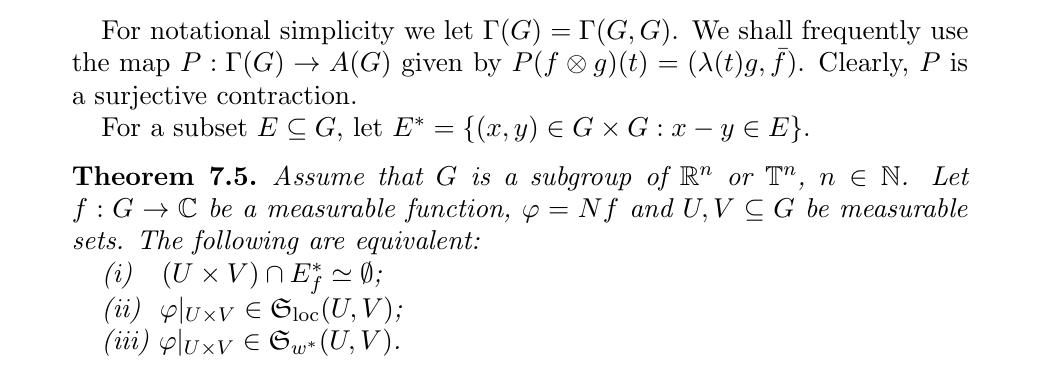
\includegraphics[width=\textwidth]{figures/theorem_context_crop.png}
\end{center}

We recall the minimum notation needed to state it.  For measurable
\(f:G\to\CC\), put
\[
                       Nf(x,y)=f(x-y).
\]
The source associates to \(f\) a closed obstruction set \(E_f\subseteq G\),
and writes
\[
                 E_f^*=\{(x,y)\in G\times G:x-y\in E_f\}.
\]
A subset of \(U\times V\) is \emph{marginally null} if it is contained in
\((M\times V)\cup(U\times N)\) for null sets \(M\subseteq U\) and
\(N\subseteq V\); the notation \(\simeq\varnothing\) means marginal
nullity.  The classes \(\Sloc(U,V)\) and \(\Sw(U,V)\) are, respectively,
the local Schur multipliers and the weak-star closable multipliers of the
source paper.

For finite-measure measurable \(A,B\subseteq G\), the elementary tensor
\(\mathbf1_A\otimes\mathbf1_B\) lies in
\(\Gamma(G)=L^2(G)\widehat\otimes L^2(G)\).  The source's contraction
\(P:\Gamma(G)\to A(G)\) satisfies
\begin{equation}\label{eq:Pindicator}
 P(\mathbf1_A\otimes\mathbf1_B)(s)
   =\mu\bigl(A\cap(B+s)\bigr).
\end{equation}

\section*{Proof Intuition}

The source already proves \((i)\Rightarrow(ii)\Rightarrow(iii)\) using only
the standing second-countable LCA hypotheses.  In the reverse implication it
also proves, without Euclidean structure, that weak-star closability forces
\[
 E_f\subseteq \nul P(\Gamma(U,V)).
\]
The only remaining task is to find conull \(U_0\subseteq U\) and
\(V_0\subseteq V\) such that no difference \(u-v\), with
\((u,v)\in U_0\times V_0\), lies in this common zero set.  Euclidean density
balls do that in the source.

On a general second-countable LCA group, choose a nonnegative normalized
\(L^1\) approximate identity.  After a common subsequence, convolution with
this approximate identity converges pointwise almost everywhere on every
finite-measure piece in countable exhaustions of \(U\) and \(V\).  At a good
pair \((u,v)\), both translated indicator averages eventually exceed
\(1/2\).  Since the averaging kernel has mass one, the two translated sets
must overlap in positive measure.  Formula~\eqref{eq:Pindicator} then gives a
tensor whose \(P\)-value at \(u-v\) is positive.  This provides exactly the
Cartesian-product, rather than merely product-almost-everywhere,
nonvanishing needed by marginal nullity.

\section*{Main Result}

\begin{theorem}\label{thm:main}
Let \(G\) be a second-countable locally compact abelian group, let
\(f:G\to\CC\) be measurable, put \(\varphi=Nf\), and let
\(U,V\subseteq G\) be measurable.  The following are equivalent:
\begin{enumerate}
\item \((U\times V)\cap E_f^*\simeq\varnothing\);
\item \(\varphi|_{U\times V}\in\Sloc(U,V)\);
\item \(\varphi|_{U\times V}\in\Sw(U,V)\).
\end{enumerate}
Consequently Theorem~7.5 of the source paper holds throughout the standing
second-countable LCA category, giving an affirmative answer to Problem~2.
\end{theorem}

\section*{The Approximate-Identity Density Lemma}

For measurable \(U,V\subseteq G\), let \(\Gamma(U,V)\) denote the subspace
of \(\Gamma(G)\) whose elementary tensors have first factor supported in
\(U\) and second factor supported in \(V\), and put
\[
                  Z_{U,V}=\nul P(\Gamma(U,V)).
\]

\begin{lemma}\label{lem:density}
For arbitrary measurable \(U,V\subseteq G\), there exist conull measurable
subsets \(U_0\subseteq U\) and \(V_0\subseteq V\) such that
\[
                       (U_0-V_0)\cap Z_{U,V}=\varnothing.
\]
More precisely, for every \(u\in U_0\) and \(v\in V_0\), there are
finite-measure sets \(U_k\subseteq U\) and \(V_l\subseteq V\) such that
\[
                  \mu\bigl(U_k\cap(V_l+u-v)\bigr)>0.
\]
\end{lemma}

\begin{proof}
Second countability and local compactness make \(G\) sigma-compact and its
Haar measure sigma-finite.  Choose increasing finite-measure exhaustions
\[
             U_1\subseteq U_2\subseteq\cdots\subseteq U,
             \qquad
             V_1\subseteq V_2\subseteq\cdots\subseteq V
\]
whose unions agree with \(U\) and \(V\) modulo null sets.

There is a sequence \((a_n)\subseteq L^1(G)\) such that
\[
 a_n\geq0,\qquad \int_Ga_n\,d\mu=1,
 \qquad T_nh:=a_n*h\longrightarrow h\quad\text{in }L^1(G)
\]
for every \(h\in L^1(G)\).  This standard sequential approximate identity
can be seen directly: take normalized indicators of a countable shrinking
base of relatively compact identity neighborhoods.  Strong continuity of
translations in \(L^1\) gives
\[
 \norm{a_n*h-h}_1
 \leq\int_G a_n(t)\norm{h(\,\cdot-t)-h}_1\,d\mu(t)
 \longrightarrow0.
\]

Enumerate the countable family
\[
 \mathcal H=\{\mathbf1_{U_k}:k\geq1\}
             \cup\{\mathbf1_{V_l}:l\geq1\}
             =\{h_1,h_2,\ldots\}.
\]
Choose a strictly increasing subsequence \(n_j\) such that
\begin{equation}\label{eq:summable}
        \sum_{m=1}^{j}\norm{T_{n_j}h_m-h_m}_1\leq2^{-j}.
\end{equation}
For fixed \(m\), summing \eqref{eq:summable} over \(j\geq m\) and using
Tonelli's theorem shows that
\[
             T_{n_j}h_m(x)\longrightarrow h_m(x)
             \quad\text{for almost every }x\in G.
\]
Thus one and the same subsequence works almost everywhere for every member
of \(\mathcal H\).

Let \(U_k^0\subseteq U_k\) and \(V_l^0\subseteq V_l\) be the corresponding
full-measure convergence sets, and set
\[
                         U_0=\bigcup_{k\geq1}U_k^0,
                         \qquad
                         V_0=\bigcup_{l\geq1}V_l^0.
\]
These are conull in \(U\) and \(V\).  Fix \(u\in U_0\) and \(v\in V_0\),
and choose \(k,l\) with \(u\in U_k^0\), \(v\in V_l^0\).  Writing
\(b_j=a_{n_j}\), for all sufficiently large \(j\) we have
\begin{align}
 \int_G b_j(t)\mathbf1_{U_k}(u-t)\,d\mu(t)&>\frac12,\label{eq:halfU}\\
 \int_G b_j(t)\mathbf1_{V_l}(v-t)\,d\mu(t)&>\frac12.\label{eq:halfV}
\end{align}
Put \(\alpha(t)=\mathbf1_{U_k}(u-t)\) and
\(\beta(t)=\mathbf1_{V_l}(v-t)\).  Since
\(\alpha+\beta\leq1+\alpha\beta\), equations
\eqref{eq:halfU}--\eqref{eq:halfV} and \(\int b_j=1\) imply
\[
 0<\int_G b_j(t)\alpha(t)\beta(t)\,d\mu(t).
\]
Hence the set
\[
 D=\{t:u-t\in U_k,\ v-t\in V_l\}
\]
has positive Haar measure.  Translation invariance, with \(x=u-t\), now
gives
\[
 \mu\bigl(U_k\cap(V_l+u-v)\bigr)=\mu(D)>0.
\]
Because \(U_k\) and \(V_l\) have finite measure,
\(\mathbf1_{U_k}\otimes\mathbf1_{V_l}\in\Gamma(U,V)\); by
\eqref{eq:Pindicator}, its \(P\)-value at \(u-v\) is positive.  Therefore
\(u-v\notin Z_{U,V}\), proving the lemma.
\end{proof}

\section*{Proof of Theorem \ref{thm:main}}

\begin{proof}
The proof of Theorem~7.5 in \cite{STT} establishes
\((i)\Rightarrow(ii)\Rightarrow(iii)\) under the standing
second-countable LCA hypotheses; no Euclidean density theorem is used in
those implications.

Assume (iii).  Before invoking density points, the source proof establishes
\begin{equation}\label{eq:sourceReduction}
                         E_f\subseteq Z_{U,V}
                         =\nul P(\Gamma(U,V)).
\end{equation}
This step uses the density of the domain of the adjoint weak-star-closable
multiplier and the source's identity \(fP(h)=P((Nf)h)\), but no special
structure of \(G\).

Apply Lemma~\ref{lem:density}.  It gives conull
\(U_0\subseteq U\), \(V_0\subseteq V\) such that
\((U_0-V_0)\cap Z_{U,V}=\varnothing\).  In view of
\eqref{eq:sourceReduction},
\[
                         (U_0-V_0)\cap E_f=\varnothing.
\]
Equivalently, \((U\times V)\cap E_f^*\) is marginally null, which is (i).
This completes the only implication left to prove.
\end{proof}

\section*{Verification Notes}

The proof was audited against pages 26--28 of the source PDF.  The authors
state in Remark~7.6(i) that the subgroup-of-\(\R^n\)-or-\(\T^n\) assumption
is used only in \((iii)\Rightarrow(i)\), at the density-point step.  The
packet changes only that step.

The edge cases were checked as follows:
\begin{enumerate}
\item potentially infinite-measure \(U,V\) are handled by finite-measure
exhaustions, ensuring the indicator tensors lie in \(L^2\widehat\otimes L^2\);
\item the summable-error choice \eqref{eq:summable} produces one common
subsequence for all exhaustion pieces;
\item the conclusion holds on a Cartesian product of conull sets, the exact
strength required for marginal nullity;
\item the sign and translation in \eqref{eq:Pindicator} agree with the
source convention \(P(\mathbf1_U\otimes\mathbf1_V)(s)
=\mu(U\cap(V+s))\);
\item no metric, doubling, or differentiation-basis assumption remains.
\end{enumerate}
No computational experiment is used or needed.

\section*{Novelty Check, Scope, and Limitations}

On August 9, 2026, bounded searches were run in arXiv and general web
indexes for the exact source title, ``Theorem 7.5,'' ``Problem 2,''
``w*-closable multiplier,'' ``local Schur multiplier,'' and combinations
with locally compact abelian groups and approximate identities.  The searches
found the source and the same authors' later arXiv:1401.2620 on closable
multipliers on group algebras.  The later paper was inspected: its principal
results concern multipliers on reduced group \(C^*\)-algebras and group von
Neumann algebras, not the restricted \(U\times V\) equivalence here.  No
later solution of Problem~2 or this argument was located.  The run's cheap
indexes likewise had no prior packet for arXiv:1001.4638.  Novelty confidence
is moderate pending a specialist citation search.

The result covers every group in Section 7's standing category:
second-countable LCA groups.  The paper develops its multiplier theory over
standard measure spaces, so non-second-countable LCA groups are outside the
literal framework used there and are not claimed in this packet.  The result
answers only Problem~2; the other four source problems are unaffected.

\section*{Human-Review Recommendation}

Recommend expert verification as a candidate full solution.  The principal
review points are:
\begin{enumerate}
\item the common-subsequence construction in Lemma~\ref{lem:density};
\item the positive-overlap inference from two averages exceeding \(1/2\);
\item the orientation of \(P\) and the finite-measure tensor placement;
\item the source-proof audit leading to \eqref{eq:sourceReduction};
\item the interpretation of Problem~2 within Section 7's standing
second-countability hypothesis.
\end{enumerate}

\begin{thebibliography}{9}

\bibitem{STT}
V.~S. Shulman, I.~G. Todorov, and L.~Turowska,
\emph{Closable Multipliers},
Integral Equations and Operator Theory \textbf{69} (2011), 29--62,
\href{https://arxiv.org/abs/1001.4638}{arXiv:1001.4638},
\href{https://doi.org/10.1007/s00020-010-1819-2}
{doi:10.1007/s00020-010-1819-2}.

\end{thebibliography}

\end{document}
